\chapter{Projekt}

\section{Abstract}
\label{abstract}


\chapter{Einleitung}
Im Seminar ``Concurrent C Programming'' welches als Vertiefung zum Kurs Systemsoftware und Betriebssystemprogrammierung gedacht ist, wurde die Aufgabe gestellt, ein Multiuser und Netwerkfähiges Client/Server Spiel in C zu entwickeln.

Ziel des Spiels ist es alle Felder dies Spielfelds zu besitzen. Das Spielfeld ist ein Quadrat der Seitenlänge $n$, wobei $$n \geq  4$$ ist. Die Koordinaten des Spielfeldes sind somit $$(0..(n-1), 0..(n-1))$$.

\section{Spielablauf}
\begin{enumerate}
	\item Der Server startet und wartet auf $\frac{n}{2}$ Spieler
	\item Sobald $\frac{n}{2}$ Spieler verbunden sind, kann jeder Spieler versuchen Felder zu erobern
	\item Es können während des Spiels neue Spieler hinzukommen oder Spieler das Spiel verlassen
	\item Der Server prüft alle $y$ Sekunden den konsistenten Spielfeldstatus , wobei $$1 \leq y \leq 30$$
	\item Wenn ein Spieler zu diesem Zeitpunkt alle Felder besitzt, hat er gewonnen und das Spiel wird beendet
\end{enumerate}

\section{Spiel-Protokol}
\begin{itemize}
	\item Befehle werden mit \textbackslash n abgeschlossen.
	\item Kein Befehl ist länger als 256 Zeichen inklusive dem \textbackslash n.
	\item Jeder Spieler kann nur 1 Kommando senden und muss auf die Antwort warten.
\end{itemize}

\subsection{Anmeldung}
\begin{lstlisting}[language=bash,caption={Erfolgreiche Anmeldung}]
Client: HELLO\n
Server: SIZE n\n	
\end{lstlisting}

\begin{lstlisting}[language=bash,caption={Nicht erfolgreiche Anmeldung}]
Client: HELLO\n
Server: NACK\n
    -> Trennt die Verbindung
\end{lstlisting}

\subsection{Spielstart}
\label{spielstart}
Der Server wartet auf $\frac{n}{2}$ Verbindungen vor dem Start.
\begin{lstlisting}[language=bash,caption={Spielstart}]
Server: START\n
Client: - (erwidert nichts, weiss das es gestartet hat)
\end{lstlisting}

\subsection{Feld erobern}
Wenn kein anderer Client gerade einen TAKE Befehl für das selbe Feld sendet, kann ein Client es nehmen.
\begin{lstlisting}[language=bash,caption={Erfolgreiche Eroberung}]
Client: TAKE X Y NAME\n
Server: TAKEN\n
\end{lstlisting}

Wenn ein oder mehrere andere Clients gerade einen TAKE Befehl für das selbe Feld sendet, sind alle bis auf der erste nicht erfolgreich.

\begin{lstlisting}[language=bash,caption={Nichterfolgreiche Eroberung}]
Client: TAKE X Y NAME\n
Server: INUSE\n
\end{lstlisting}

\subsection{Besitz anzeigen}
\begin{lstlisting}[language=bash,caption={Spielstart}]
Client: STATUS X Y\n
Server: Name-des-Spielers\n
\end{lstlisting}

\subsection{Spielende}
Sobald ein Client alle Felder besitzt wird der Gewinner bekanntgegeben. Diese Antwort kann auf jeden Client Befehl kommen, mit Ausnahme der Anmeldung kommen.
\begin{lstlisting}[language=bash,caption={Spielstart}]
Server: END Name-des-Spielers\n
Client: - (beendet sich)
\end{lstlisting}

\section{Bedingungen für die Implementation}
\begin{itemize}
	\item Es gibt keinen globalen Lock
	\item Der Server speichert den Namen des Feldbesitzers
	\item Kommunikation via TCP/IP
	\item fork + shm (empfohlen)
	\begin{itemize}
		\item oder pthreads
		\item für jede Verbindung einen prozess/thread
		\item Hauptthread/prozess kann bind/listen/accept machen
		\item Rating Prozess/Thread zusätzlich im Server
	\end{itemize}
	\item Fokus liegt auf dem Serverteil
	\item Client ist hauptsächlich zum Testen und "Spass haben" da
	\item Server wird durch Skript vom Dozent getestet
	\item Locking, gleichzeitiger Zugriff im Server lösen
	\item Debug-Ausgaben von Client/Server auf stderr
\end{itemize}

\chapter{Planung und Implementation}
Bevor mit der Implementation begonnen wurde, wurden die Anforderungen analysiert und den Spielablauf mit einem simplen Blocks-and-Arrows Diagram zu Papier gebracht.

Mit dieser Visualisierung konnte im nächsten Schritt die Anforderungen an den Server ermittelt werden. Danach wurde ein weiteres Diagram angefertigt, welches die Funktionalität des Servers und die Abhängigkeiten der einzelnen Komponenten des Servers aufzeigt, siehe Abbildung \ref{fig:server}.

\begin{figure}[!ht]
  %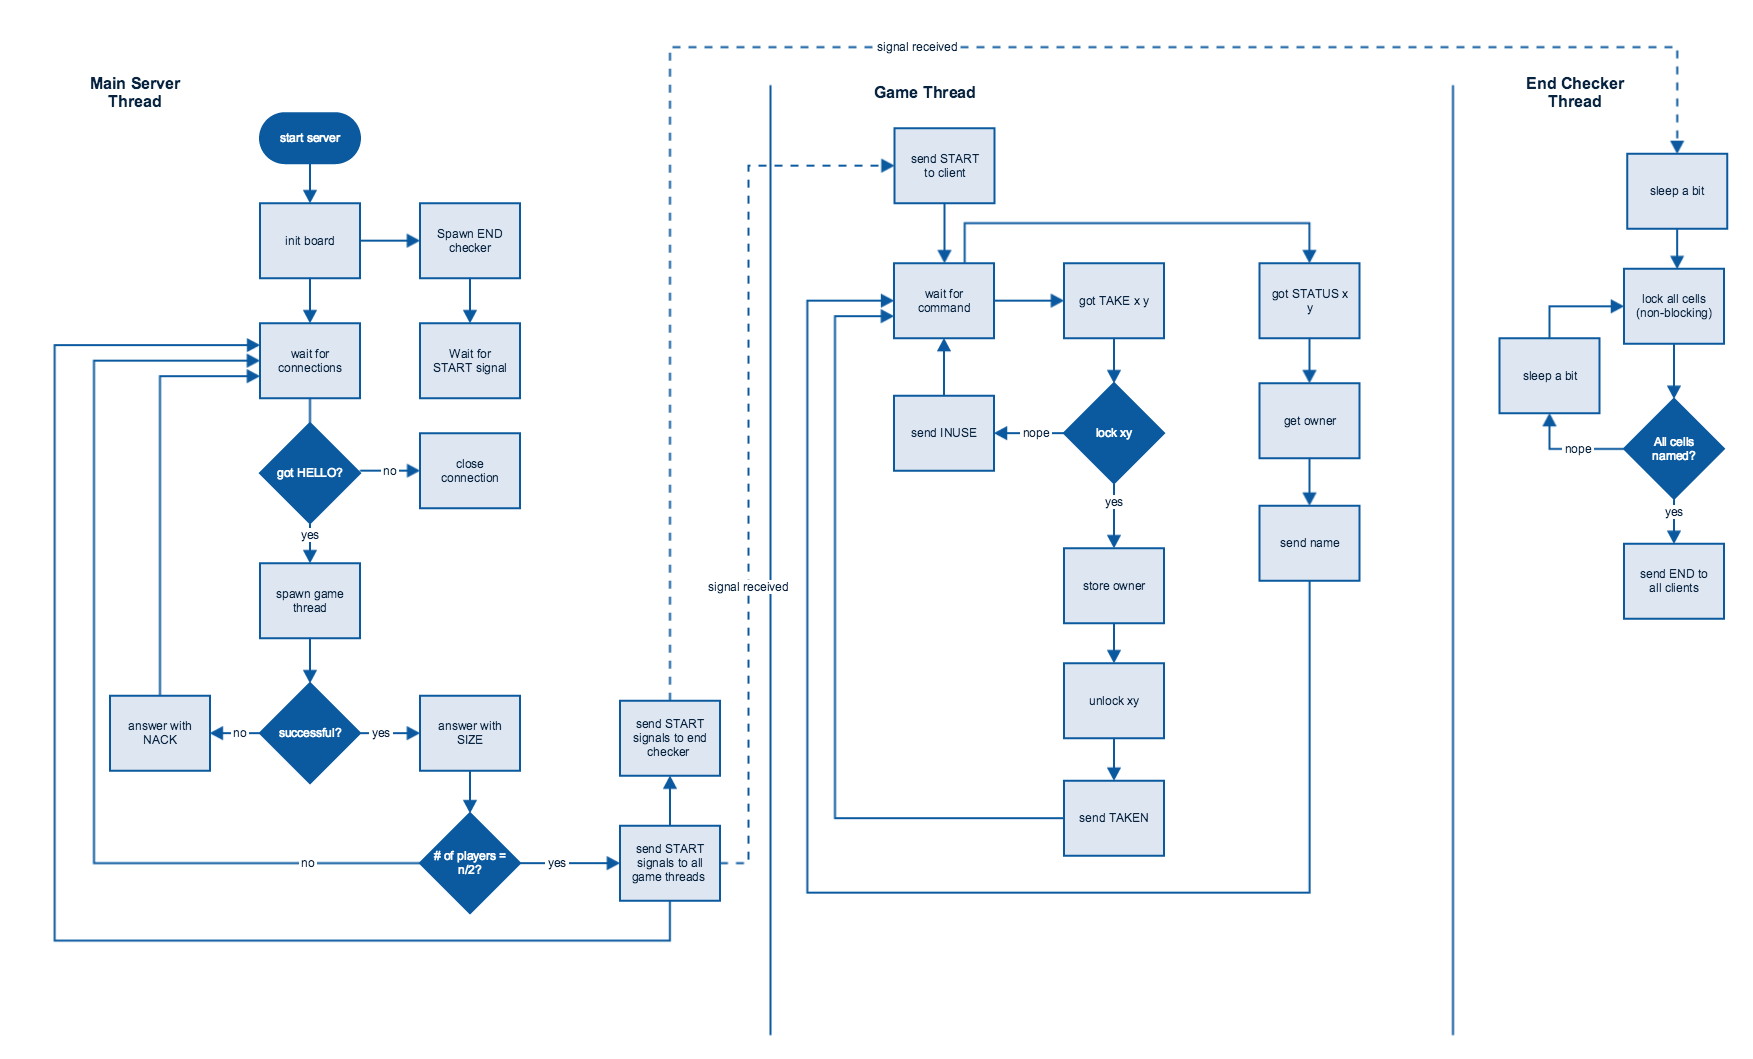
\includegraphics[width=\textwidth,height=\textheight,keepaspectratio]	{images/server}
  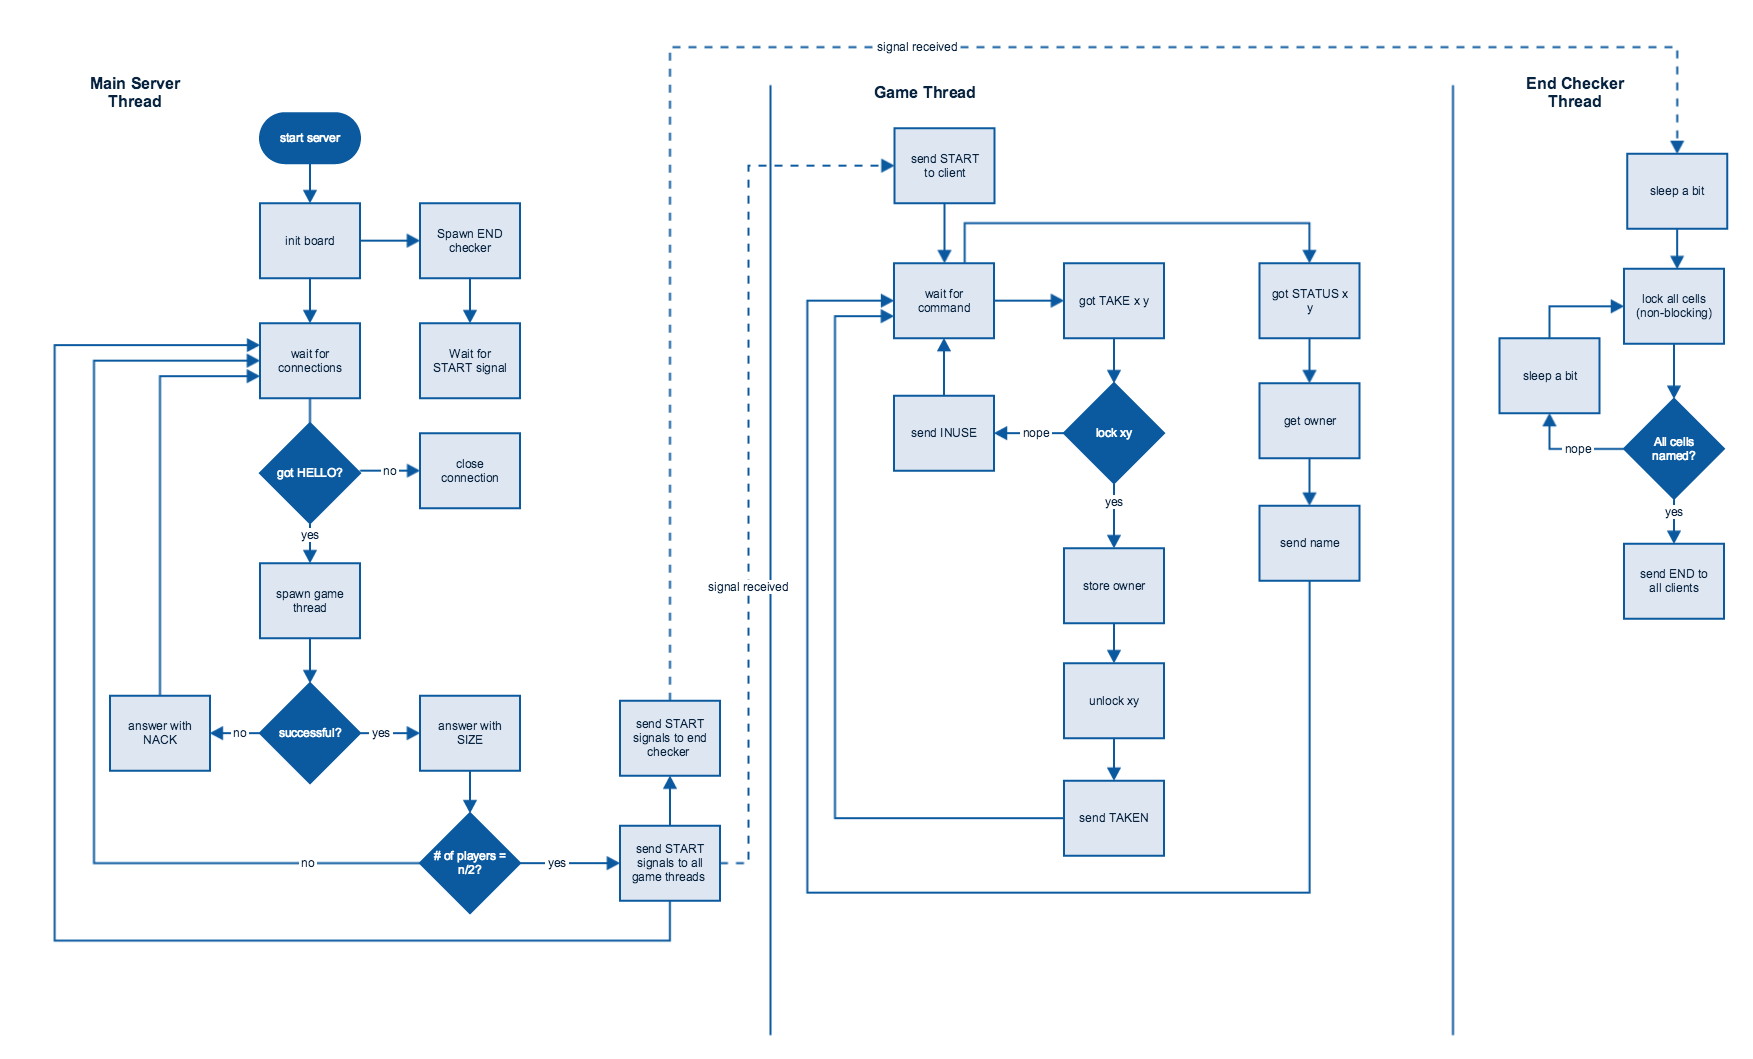
\includegraphics[max size={\textwidth}{\textheight}]{images/server}
  \caption{\label{fig:server}Server}
\end{figure}

Das Erstellen dieses Diagrams beanspruchte einiges an Zeit und war ein iterativer Prozess, weil nach jeder Version neue Fallstricke ersichtlich wurden. Doch die Arbeit lohnte sich, da die Grafik die Implementation enorm vereinfachte weil es klar ersichtlich wurde, was welche Komponente zu erfüllen hat.

\section{Server}
Wie Abbildung \ref{fig:server} zu entnehmen ist, besteht der Server aus drei Hauptkomponenten:
\begin{itemize}
	\item Main Server Thread
	\item Game Thread
	\item End Checker Thread
\end{itemize}

\subsection{Main Server Thread}
Der Main Server Thread ist verantwortlich den Server zu starten und neue Verbindungen anzunehmen und zu speichern. Sobald genügend Clients verbunden sind, soll er auch die START Nachricht wie in \ref{spielstart} definiert an alle Clients versenden.

Beim Starten des Servers wird als erstes die Umgebung aufgesetzt. Das beinhaltet neben dem Registrieren der Signal-Handlern auch das initialisieren des Logging Frameworks, dem Verarbeiten der Kommandozeilenparametern und dem Setup des Spielfeldes. Um allen Clients den Start-Befehl zur selben Zeit zu schicken, wird eine PThread-Barriere verwendet und auch am Anfang initialisiert.

Sind all diese Schritte erfolgreich abgeschlossen, wird ein neuer Thread erstellt welcher die eingehenden Verbindungen verarbeiten wird. 

\subsubsection{Connection Handler}
Der Connection Handler basiert auf den Erklärungen von \cite{byte-stream-server}. Wenn eine neue Verbindung zum Server erstellt wird, wird dieser ein neuer File Descriptor zugewiesen. 	Danach wird ein neues Spieler struct erstellt und der File Descriptor wird darin gespeichert. Nun ist die Verbindungsinitialisierung komplett und ein Game Thread wird erstellt. Falls etwas schiefgeht wird ein NACK an den Client geschickt und die Verbindung wird terminiert.

 
\subsection{Game Thread}
Der Game Thread ist eine unendliche \texttt{while}-Schleife die mit \texttt{recv} auf einkommende Befehle hört.

Als erstes werden allfällige Steuerzeichen (\textbackslash n, \textbackslash r) aus dem Buffer entfernt und danach die Daten geparsed und die entsprechende Antwort an den Client geschickt.

Handelt es sich dabei um ein \texttt{HELLO}, wird geprüft ob sich genug Spieler am Server angemeldet haben. Falls das zutrifft, wird die Barriere aufgehoben und alle Spieler erhalten zur gleichen Zeit das \texttt{START} Kommando. Zusätzlich wird der End Checker Thread gestartet. Falls nicht genügend Spieler online sind, wartet der Thread an der Barriere bis es weitergeht. Ist das Spiel schon gestartet, wird sofort der Start Befehl ausgelöst.


\subsection{End-Checker}
Der End-Checker Thread läuft wie der Connection Handler in einer Dauerschleife bis ein Gewinner ermittelt ist. Git es einen Gewinner, schickt der End-Checker die END Nachricht.

In der Aufgabenstellung wird gefordert, dass kein globaler Lock verwendet wird. Es wird aber auch verlangt, dass das Spielfeld konsistent geprüft werden muss. Da sich diese zwei Anforderungen jedoch nicht vereinbaren lassen, habe ich mich entschieden eine Lösung ohne globalen Lock zu entwickeln. Dies hat jedoch zur Folge, dass ein Spielfeld welches am Anfang getestet wird beim Abschluss der Prüfung aller Felder einen neuen Besitzer haben kann.

Wenn das Check-Timeout abgelaufen ist, iteriert der End-Checker durch das gesamte Board und versucht die Zelle mit einem Mutex zu locken. Dabei wird ein locking-mutex verwendet, der Checker bleibt also bei jeder Zelle so lange stehen, bis er den Lock erfolgreich erhalten hat. 

Sobald der Lock erfolgreich akquiriert wurde, wird geprüft, ob der momentane Zellen Inhaber derselbe ist, wie von der Zelle vorher. Sind beide Besitzer gleich, wird mit der nächsten Zelle fortgefahren, falls nicht, wird die Überprüfung angehalten, der Lock freigegeben und wieder eine zufällige Zeit gewartet.

Falls der Checker einen Gewinner ermittelt hat, wird jedem Spieler die \texttt{END} Nachricht geschickt und der Thread beendet sich.  

\section{Client}
Der Client ist äusserst simple implementiert und beherrscht nur einen Modus.

\chapter{Fazit}
Das Projekt war äusserst interessant und hat neben viel Ärger auch sehr viel Freude bereitet. Es war das erste Projekt welches ich in C geschrieben habe, demzufolge war die Lernkurve auch ziemlich Steil. Hinzukommt, dass ich beruflich nicht Vollzeit programmiere und es schon eine Weile her war seit meinem letzten Programmier-Projekt.

Glücklicherweise ist beinahe jedes Problem schon einmal gelöst worden und es gibt ausreichend Dokumentation im Internet. Auch der Tipp mit valgrind war äusserst nützlich. 

Das Projekt zeigte mir auch deutlich warum Sprachen wie Java und C\# soviel auftrieb erhalten haben. Muss man sich doch in C jede noch so kleine Funktion in der Regel selbst bauen. Ein TCP Server in Java kann inner Minuten geschrieben werden ohne das man sich gross Gedanken machen muss, wie man es im Hintergrund abläuft.

Auch der Umgang mit dem Speicher (Speicherreservierung) hat viel Nerven gekostet - umso schöner jedoch, wenn man dann endlich auch den letzten Fehler ausgeschliffen hat!